\documentclass{beamer}
    \usetheme{Boadilla}
\usepackage{polyglossia}
    \setmainlanguage{english}
\usepackage{fontspec}
    \setsansfont{Linux Biolinum O}
\usepackage{graphicx}
\usepackage{xcolor} \usepackage{rotating}
\usepackage{listings}
    \lstset{language=bash,
	basicstyle=\footnotesize\ttfamily\tiny,
	breaklines=true,
	framextopmargin=50pt,
	frame=bottomline,
	backgroundcolor=\color{white!86!black},
	commentstyle=\color{blue},
	keywordstyle=\color{red},
	stringstyle=\color{orange!80!black}}
\usepackage{amsmath}
\usepackage{amssymb}
\usepackage[binary-units=true]{siunitx}
\usepackage{booktabs}
\usepackage{float}
\usepackage{tabularx}
\usepackage{caption}
\usepackage{subfig}
\usepackage{tikz}
    \usetikzlibrary{patterns}
    \usetikzlibrary{decorations.pathreplacing}
\usepackage{datenumber}
\setbeamertemplate{itemize items}[circle]
\usepackage{hyperref}
     \hypersetup{
     colorlinks=true,
     linkcolor=black,
     filecolor=magenta}

\title{\texorpdfstring{\color{blue!50!black}\textbf{Status Report}}{}}
\subtitle{Cosmics with the ALPIDE Telescope}
\author[Maurice \and Felicitas \and David]{Maurice Donner \and Felicitas Franke \and David Schledewitz}
\date{September 22th, 2020}

\begin{document}

\maketitle
\newpage

\begin{frame}{Back in May...}
    \begin{itemize}
	\item Limited access to GSI
	\item Set up the telescope to be pointed towards the sky and record
	    cosmics
	\item At first \textbf{no scintillators} available \\[1cm]
    \end{itemize}

\LARGE Method of operation \footnotesize \\[.5cm]

\begin{minipage}[b]{.49\textwidth}
    \begin{itemize}
	\item Use a NIM signal generator to create artificial triggers for the
	    chips.
	\item Trigger every \textasciitilde \( 100 \ \si{\micro \second} \)
	\item That way no event should be missed
    \end{itemize}
\end{minipage}
%
%\begin{minipage}[b]{.49\textwidth}
    \begin{figure}[H]
    \centering \tiny
    \begin{tikzpicture}[remember picture, overlay,yshift=1.3cm,xshift=.5cm,scale=1.3]
    % Draw Coordinate system and axis labels
    \draw[->] (0,0) -- (4,0) node[anchor=north] {t};
    \draw[->] (0,0) -- (0,1);
    \draw (0,0) node[anchor=north] {0 $\si{\micro \second}$};
    \draw (2,0) node[anchor=north] {95.8 $\si{\micro \second}$};
    % Draw Strobes
    \filldraw[fill=blue!20,draw=blue!50!black] (0,0) rectangle (1.8,0.8);
    \filldraw[fill=blue!20,draw=blue!50!black] (2,0) rectangle (3.8,0.8);
    % Draw strobe length
    \draw [decorate,decoration={brace,amplitude=3pt},xshift=0pt,yshift=1pt]
    (2.0,0.8) -- (3.8,0.8) node [black,midway,yshift=10pt] 
    {$90 \ \si{\micro \second}$ };
    % Draw Discriminator Signal
    \draw[pattern=north west lines,pattern color = red!50!black] (1.9,0) rectangle (2.1,0.8);
    \draw[pattern=north west lines,pattern color = red!50!black] (0.4,0) rectangle (0.6,0.8);
    % Draw discriminator signal length
    \draw [decorate,decoration={brace,amplitude=1pt},xshift=0pt,yshift=1pt]
    (0.4,0.8) -- (0.6,0.8) node [black,midway,yshift=5pt] 
    {$10 \ \si{\micro \second}$ };
    % Draw Legend
    \filldraw[fill=blue!20,draw=blue!50!black] (0,-0.4) rectangle (0.2,-0.6)
    node[anchor=west] {STROBE signal};
    \draw[pattern=north west lines,pattern color = red!50!black] (0,-0.8) rectangle (0.2,-1)
    node[anchor=west] {Discriminator signal};
    % Draw Trigger
    \draw[->] (2.0, 1.1) -- (2.0, 0.9) node[anchor=south,yshift=5pt] {\tiny trigger};
    \end{tikzpicture}
    \end{figure}
%\end{minipage}
\end{frame}

\begin{frame}{Back in May...}
    \Large PROs \footnotesize \\
    \begin{itemize}
	\item Running "without" external trigger possible
	\item Thin time slices makes it really unlikely to detect
	    two muons at the same time, especially from similar angles.
    \end{itemize}
    \Large CONs \footnotesize 
    \begin{itemize}
	\item $> 10 \, 000$ Events per second (mostly empty)
	\item $4.4 \ \si{\mega \byte}$ per second of Data written to the disk
	\item EUDAQ 1 crashed often at filesizes \( > 5 \ \si{\giga \byte} \)
	    $\rightarrow$ Runtime limited to \( \approx 18 \ \si{\minute} \) 
    \end{itemize}
\end{frame}

\begin{frame}{Taking Cosmics}
    Took 380 runs á 14-18 minutes in total over the course of several days
    \begin{figure}[H]
	\centering
	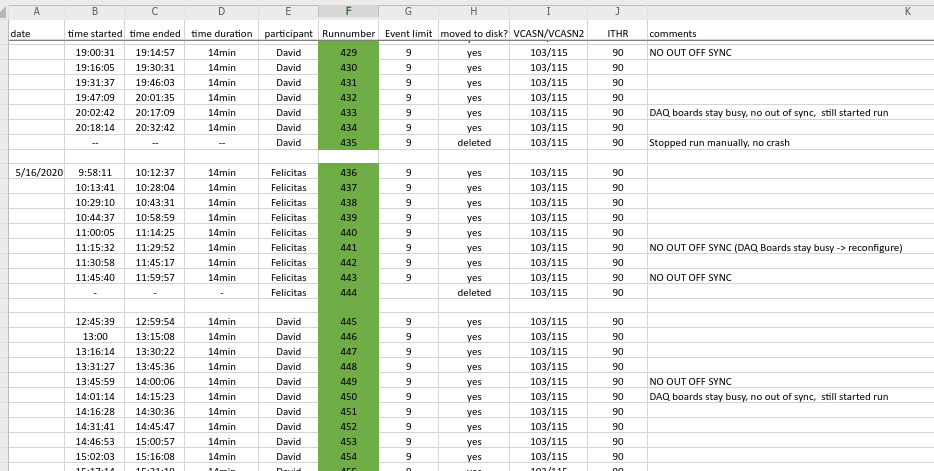
\includegraphics[width=.9\textwidth]{Screenshot.png}
    \end{figure}
    \footnotesize
    \begin{minipage}{.33\textwidth}
	\begin{itemize}
	    \item 1.5 TB of Data
	\end{itemize}
    \end{minipage}
    \begin{minipage}{.65\textwidth}
	\begin{itemize}
	    \item First Analysis showed only \textasciitilde 10 good tracks per
		run
	\end{itemize}
    \end{minipage}
\end{frame}

\begin{frame}[fragile]{Cosmic Analysis}
    \footnotesize
    \begin{itemize}
	\item Corryvreckan fails to do analysis with just a few tracks per run \\
	    \tiny (no way of using multiple \verb`.raw` files?) \footnotesize
	\item Used the \verb`[TextWriter]` module to transform RAW data into
	    \verb`.txt` files.
	\item Reducing filesize from \textasciitilde \( 4.5 \ \si{\giga \byte} \)
	    to \textasciitilde \( 200 \ \si{\mega \byte} \) per run
	\pause
	\item Compression program stores only non-empty events.
	\item Reduces size of \verb`.txt` files to \textasciitilde
	    \( 90 \ \si{\kilo \byte} \) 
	\item Further analysis in python
    \end{itemize}
\end{frame}

\begin{frame}{Cosmic Analysis}
    \footnotesize
    \begin{itemize}
	\item First visualization attempts
	\item Plane alignment with testbeam data from 2019 \( \rightarrow \)
	    inaccurate. \tiny (planes seem to have shifted) \footnotesize
    \end{itemize}
\begin{minipage}{.45\textwidth}
    \centering
    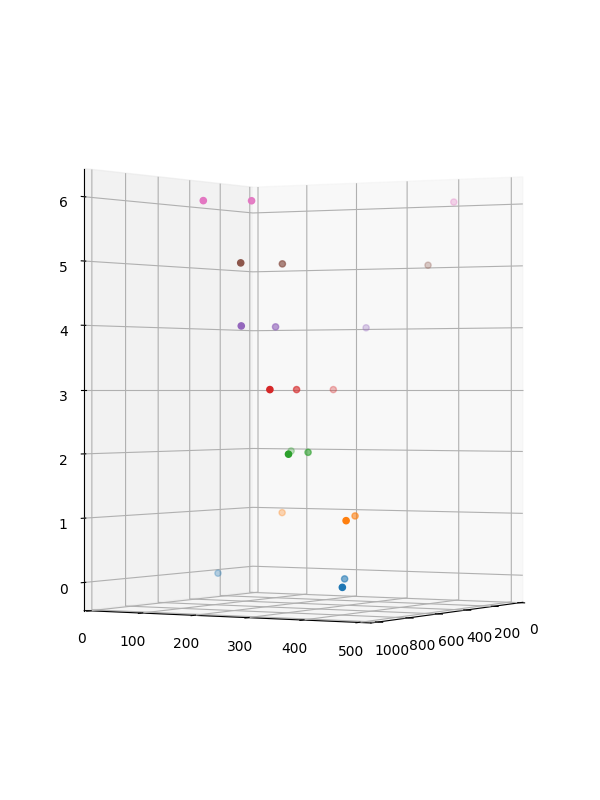
\includegraphics[trim=0 50 0 100,clip,width=\textwidth]{DESY_Before.png}
\end{minipage}
\begin{minipage}{.05\textwidth}
    \centering
    \( \rightarrow \)
\end{minipage}
\begin{minipage}{.45\textwidth}
    \centering
    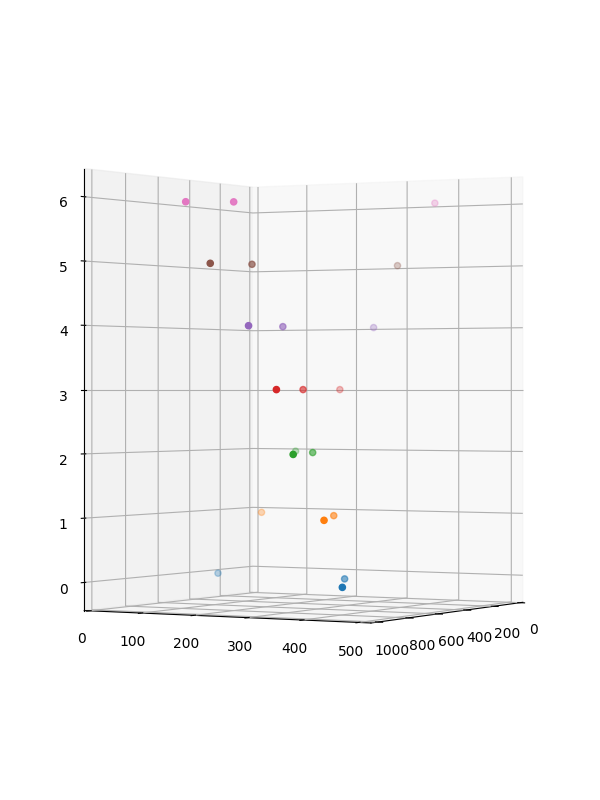
\includegraphics[trim=0 50 0 100,clip,width=\textwidth]{DESY_After.png}
\end{minipage}
\begin{itemize}
    \item Taking Closer look at alignment
\end{itemize}
\end{frame}

\begin{frame}{Cosmic Analysis}
    \footnotesize
    \begin{minipage}{.6\textwidth}
    \begin{figure}[H]
	\centering
	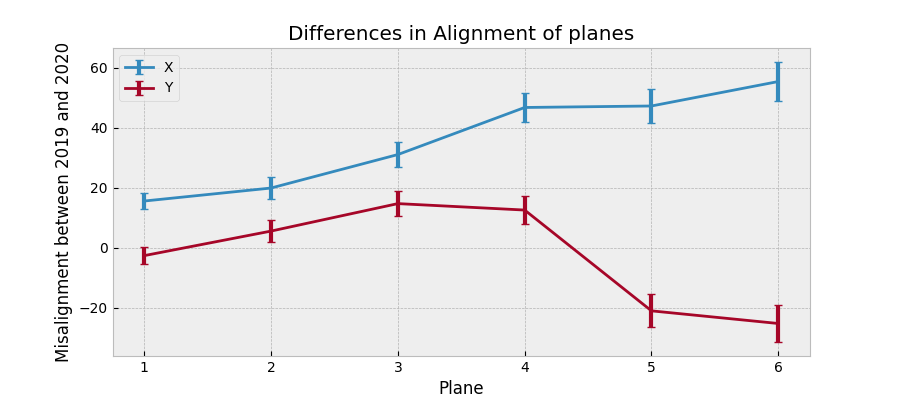
\includegraphics[trim=30 0 50 0, clip, width=\textwidth]{Misalignment.png}\\
	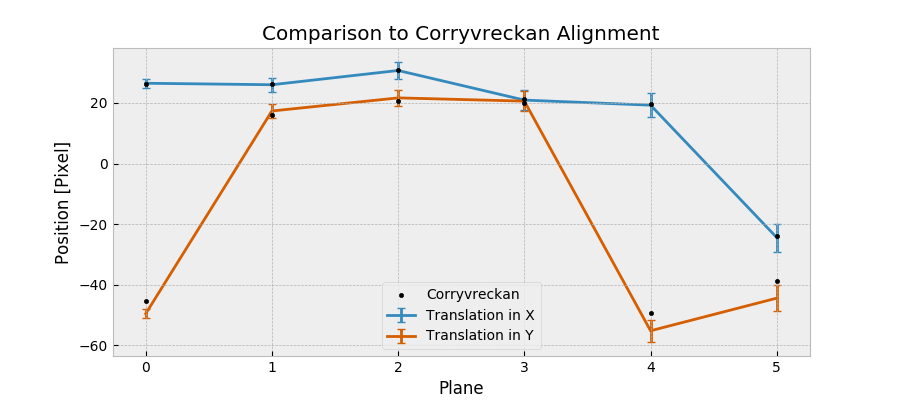
\includegraphics[trim=30 0 50 0, clip, width=\textwidth]{Corry.png}
    \end{figure}
    \end{minipage}
    \begin{minipage}{.39\textwidth}
	\begin{itemize}
	    \item Disalignment of planes to over \( 1.8 \ \si{\milli \meter} \)
		(after transport)
	    \item Generally, testbeam alignment from 2020 closer to cosmic
		setup than from 2019
	    \item simple translation algorithm and comparison with the alignment
		that corryvreckan suggests (second figure)
	    \item Goal: Do alignment with cosmic data
	\end{itemize}
    \end{minipage}
\end{frame}

\begin{frame}[fragile]{Cosmic Analysis}
    Implemented a 3D-Fitting algorithm in python:\\
    \begin{minipage}{.32\textwidth}
	\begin{figure}[H]
	    \centering
	    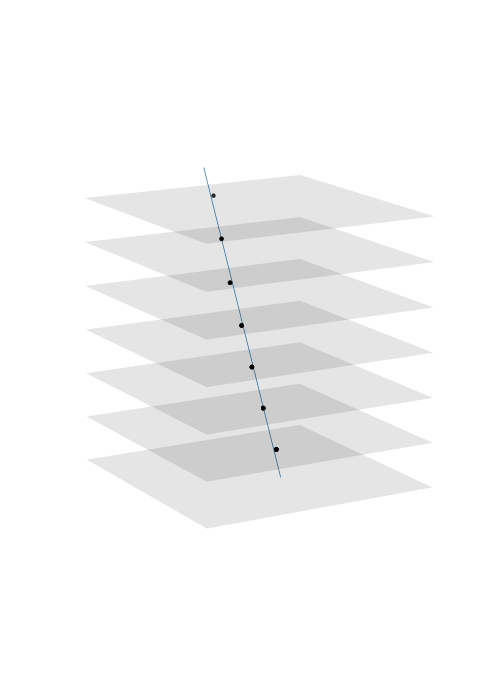
\includegraphics[trim=0 80 0 80,clip,width=\textwidth]{example_1459.png}
	\end{figure}
    \end{minipage}
    \begin{minipage}{.32\textwidth}
	\begin{figure}[H]
	    \centering
	    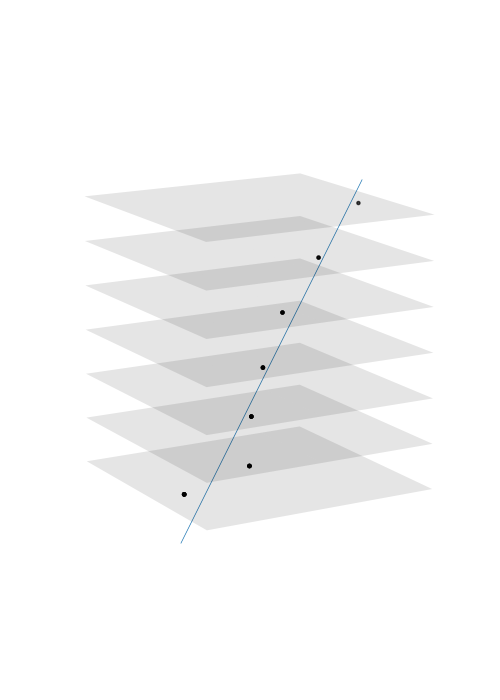
\includegraphics[trim=0 80 0 80,clip,width=\textwidth]{example_112000.png}
	\end{figure}
    \end{minipage}
    \begin{minipage}{.32\textwidth}
	\begin{figure}[H]
	    \centering
	    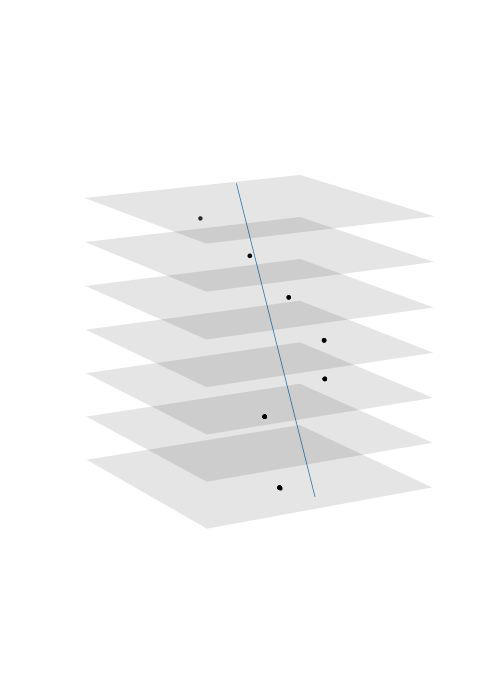
\includegraphics[trim=0 80 0 80,clip,width=\textwidth]{example_290252.png}
	\end{figure}
    \end{minipage}\\
    Using numpy's Singular value decomposition \verb]np.linalg.svd] \\[.1cm]
    \( \rightarrow \) Calculating \( \chi ^2 \) (goodness of fit) "by hand" \\
    \begin{minipage}{.4\textwidth}
	\begin{figure}[H]
	    \centering
	    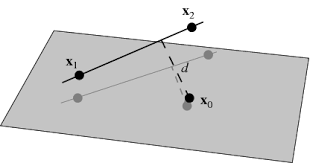
\includegraphics[width=\textwidth]{pointin3d.png}
	\end{figure}
    \end{minipage}
    \begin{minipage}{.59\textwidth}
	\footnotesize
	\begin{align*}
	    d^2 = \frac{ \left| x_1-x_0 \right|^2 \left| x_2-x_1 \right|^2
		- \left[ \left( x_1-x_0 \right) \cdot \left( x_2-x_1 \right)
		\right]^2}{\left| x_2-x_1 \right|^2}
	\end{align*}
    \end{minipage}
\end{frame}

\begin{frame}{Cosmic Analysis}
  \LARGE Event analysis \normalsize \\[.1cm]
  \begin{itemize}
    \item With simple considerations estimate muon rate traversing a certain number of planes
    \item Evaluate data and compare to estimations
  \end{itemize}
  \begin{figure}[H]
    \centering
    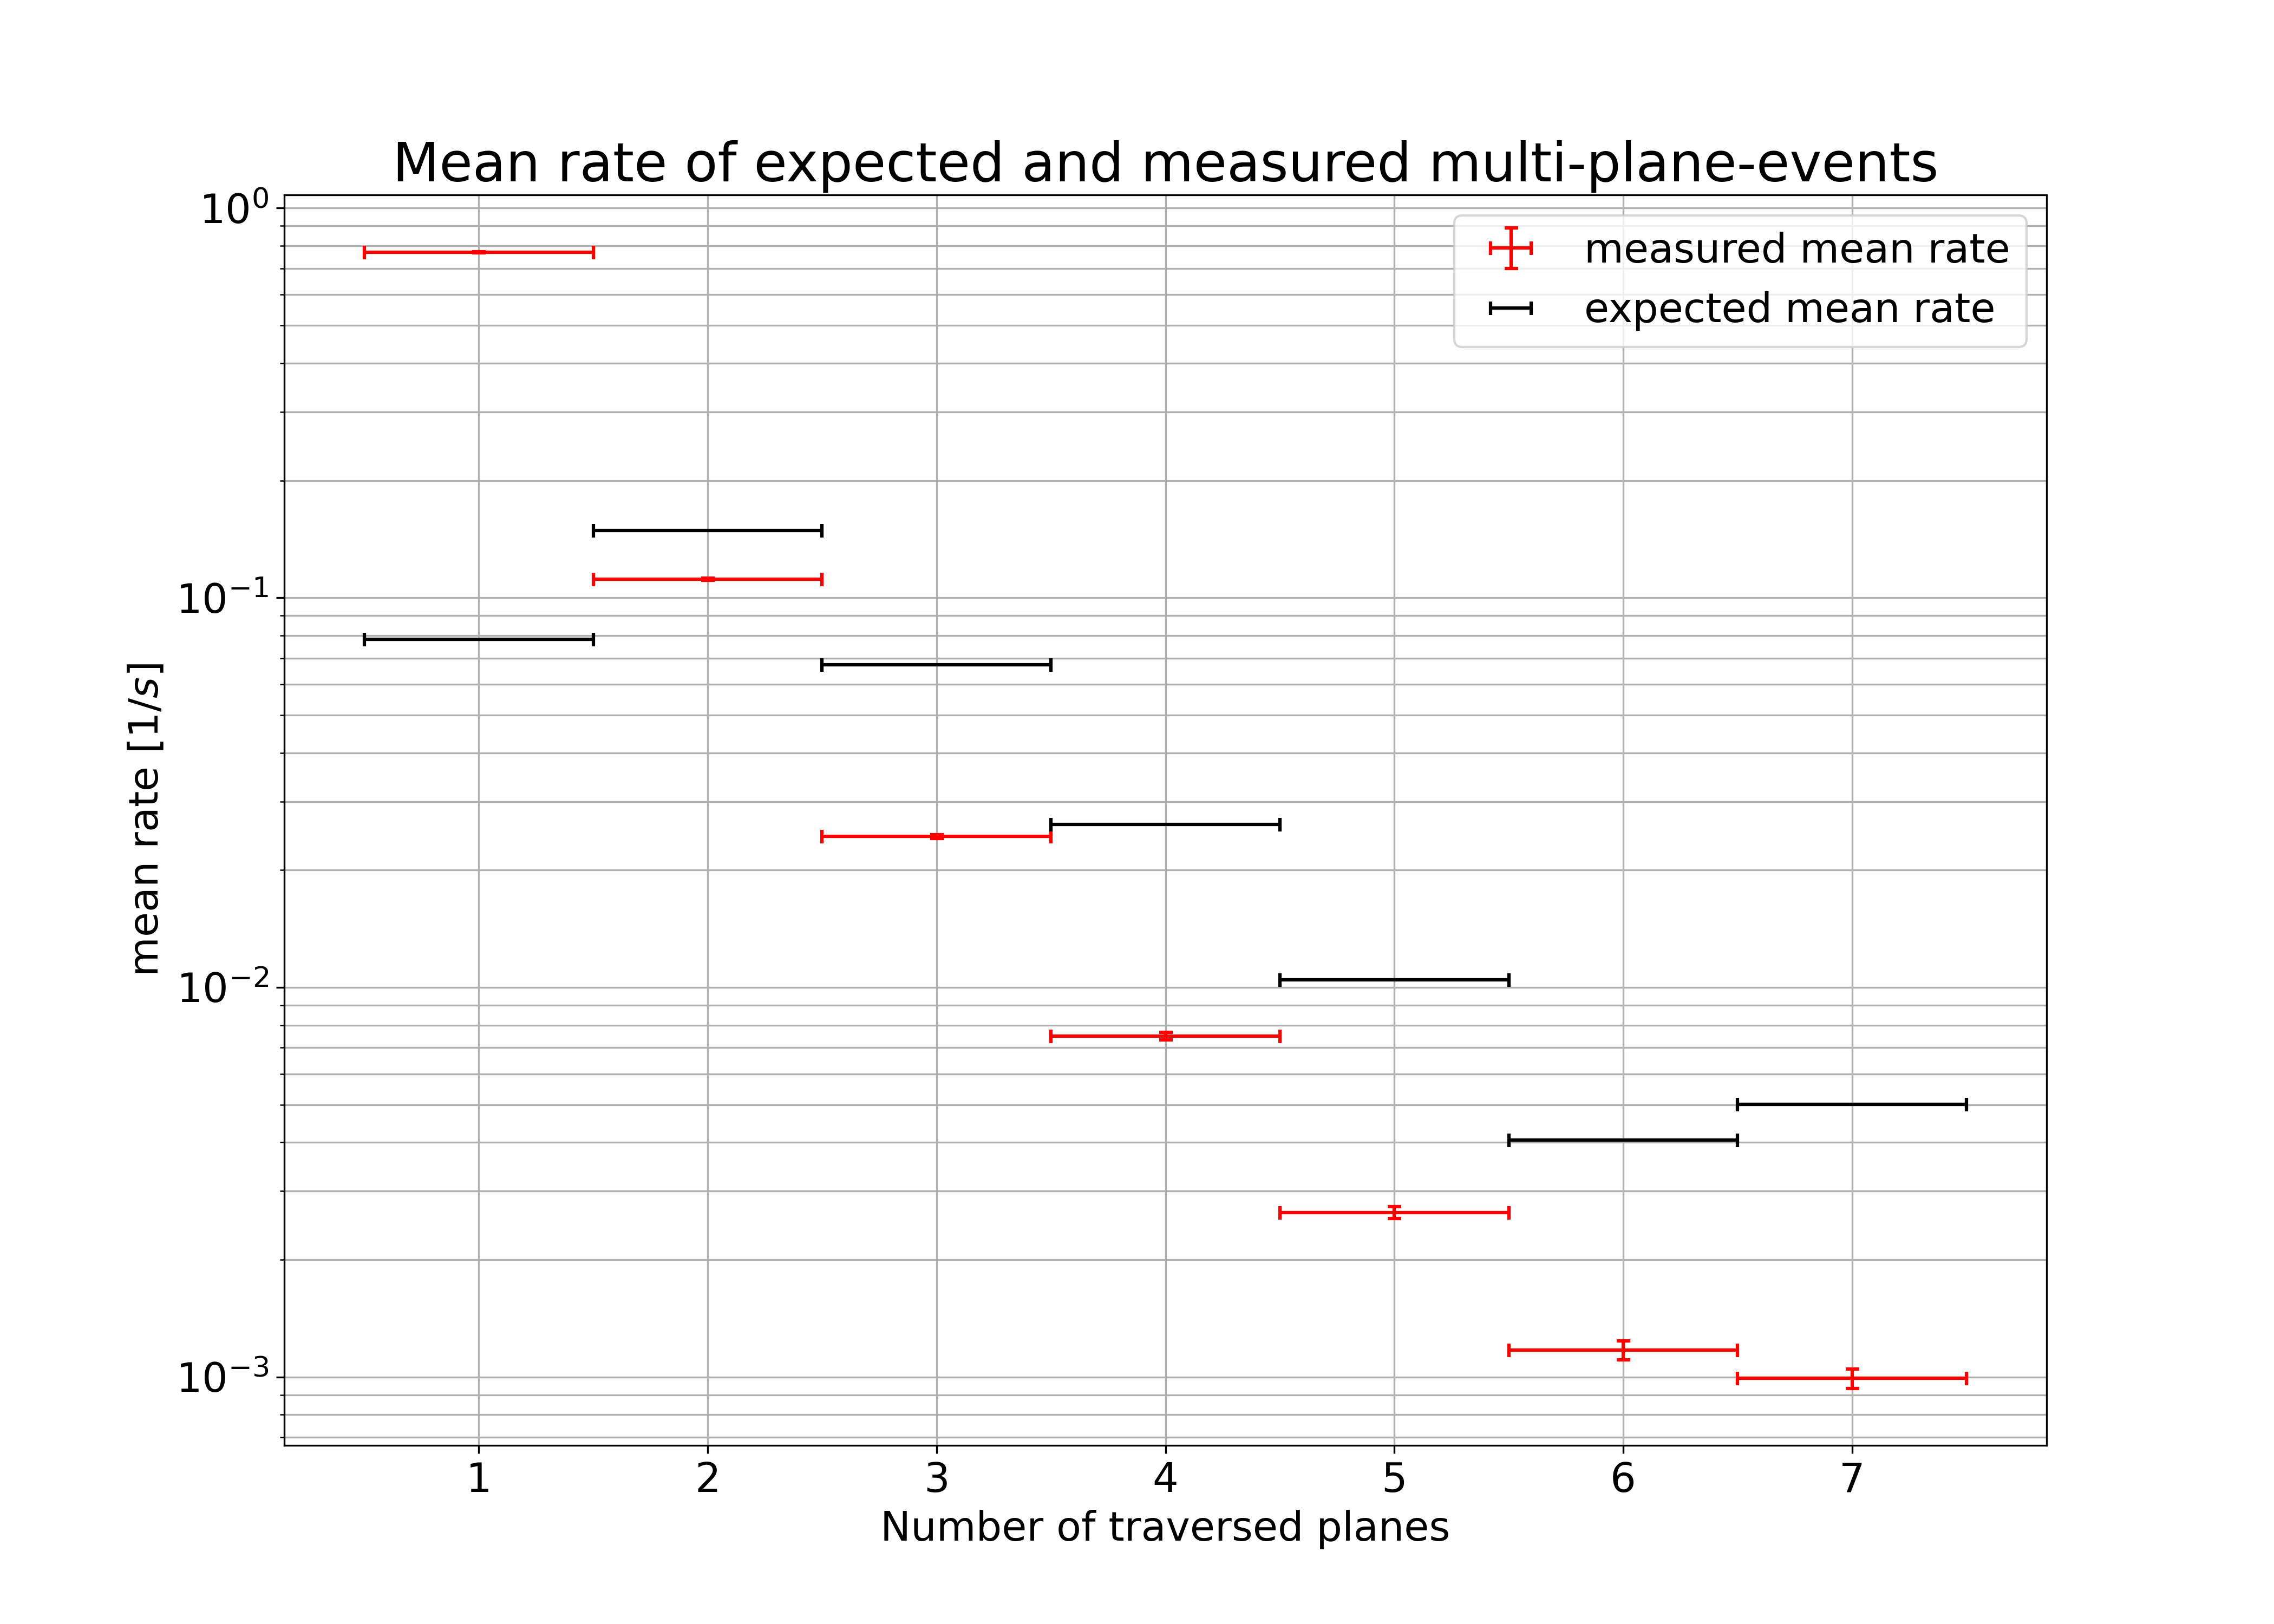
\includegraphics[width=.8\textwidth]{rate_comparison}
    \caption{Comparison of estimated and measured muon rate}
  \end{figure}
\end{frame}

\begin{frame}{June}
  \LARGE event analysis \normalsize \\[.1cm]
  \begin{itemize}
    \item Find reasons for overestimation
    \item Differences in measured hit rate per plane
    \item possible dependency on Thresholds
  \end{itemize}
  \begin{figure}[H]
    \centering
    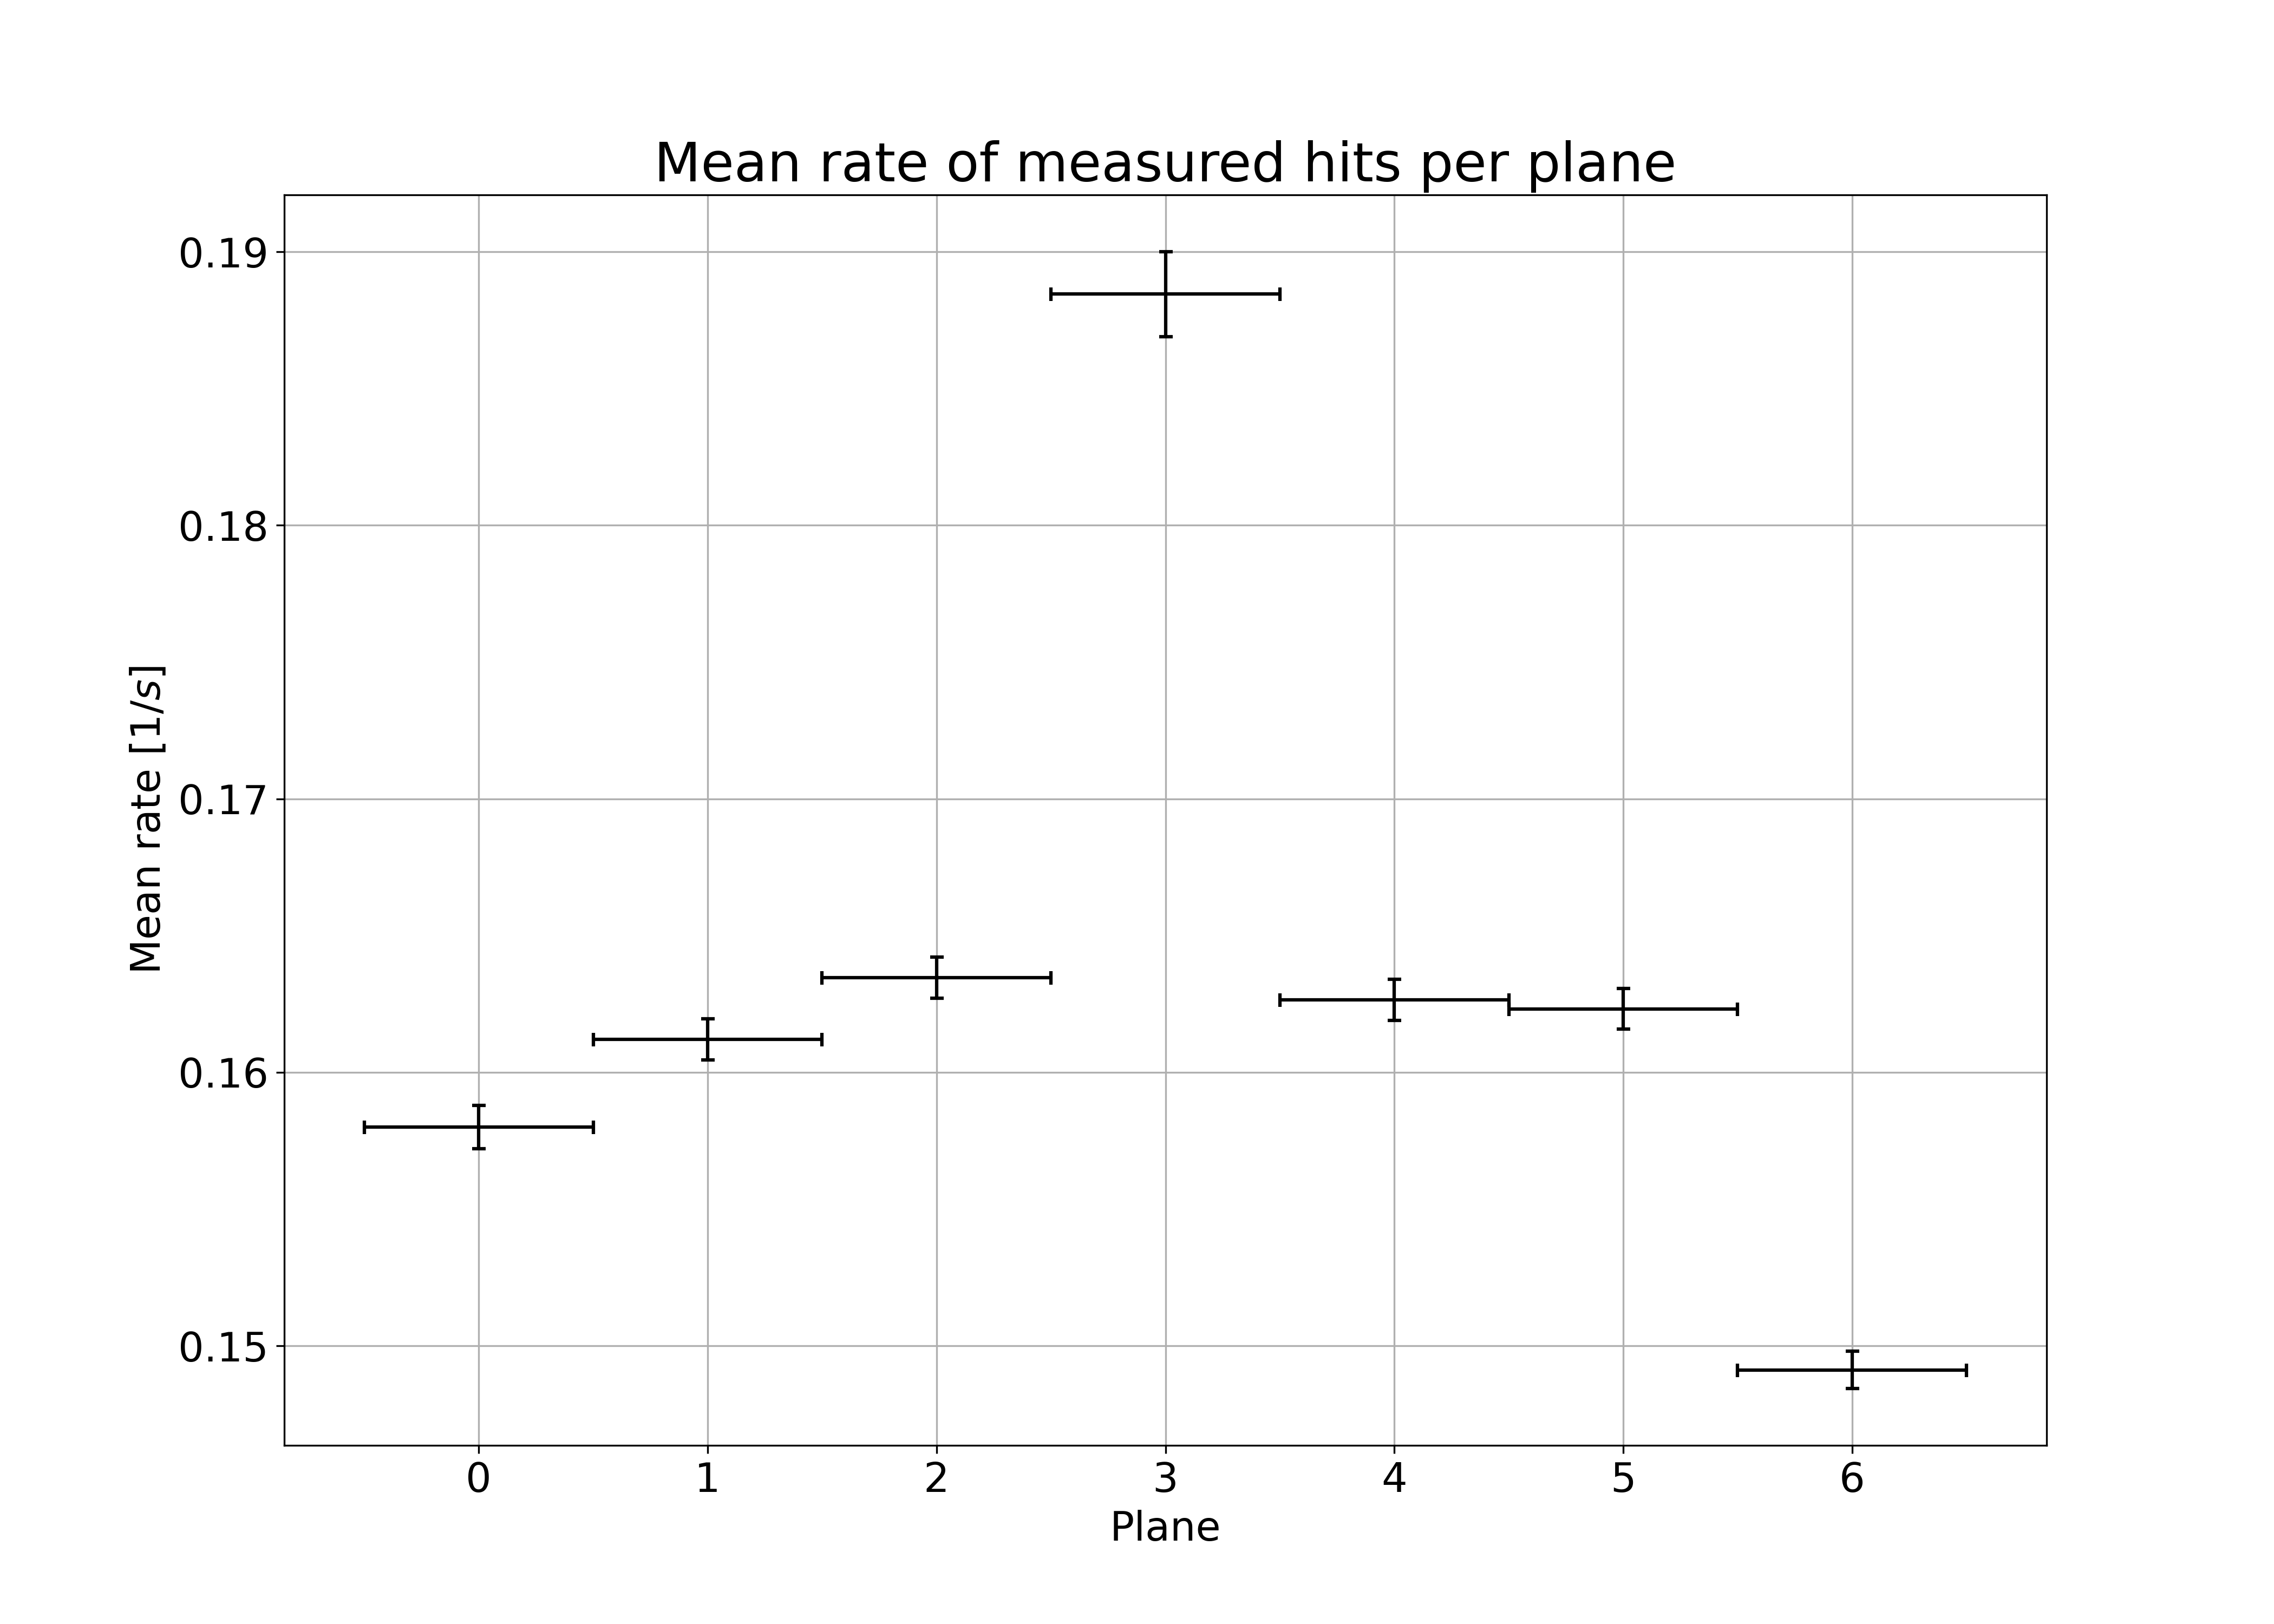
\includegraphics[width=.8\textwidth]{rate_per_plane}
    \caption{Mean rate of measured hits}
  \end{figure}
\end{frame}

\begin{frame}{Cosmic Analysis}
  \LARGE event analysis \normalsize \\[.1cm]
  \begin{itemize}
    \item Non-consecutive events appeared\\
    (i.e. planes 1,2,3,4,5,7 registered a hit)
    \item Corrected mean rate by removing non-consecutive events
  \end{itemize}
  \begin{figure}[H]
    \centering
    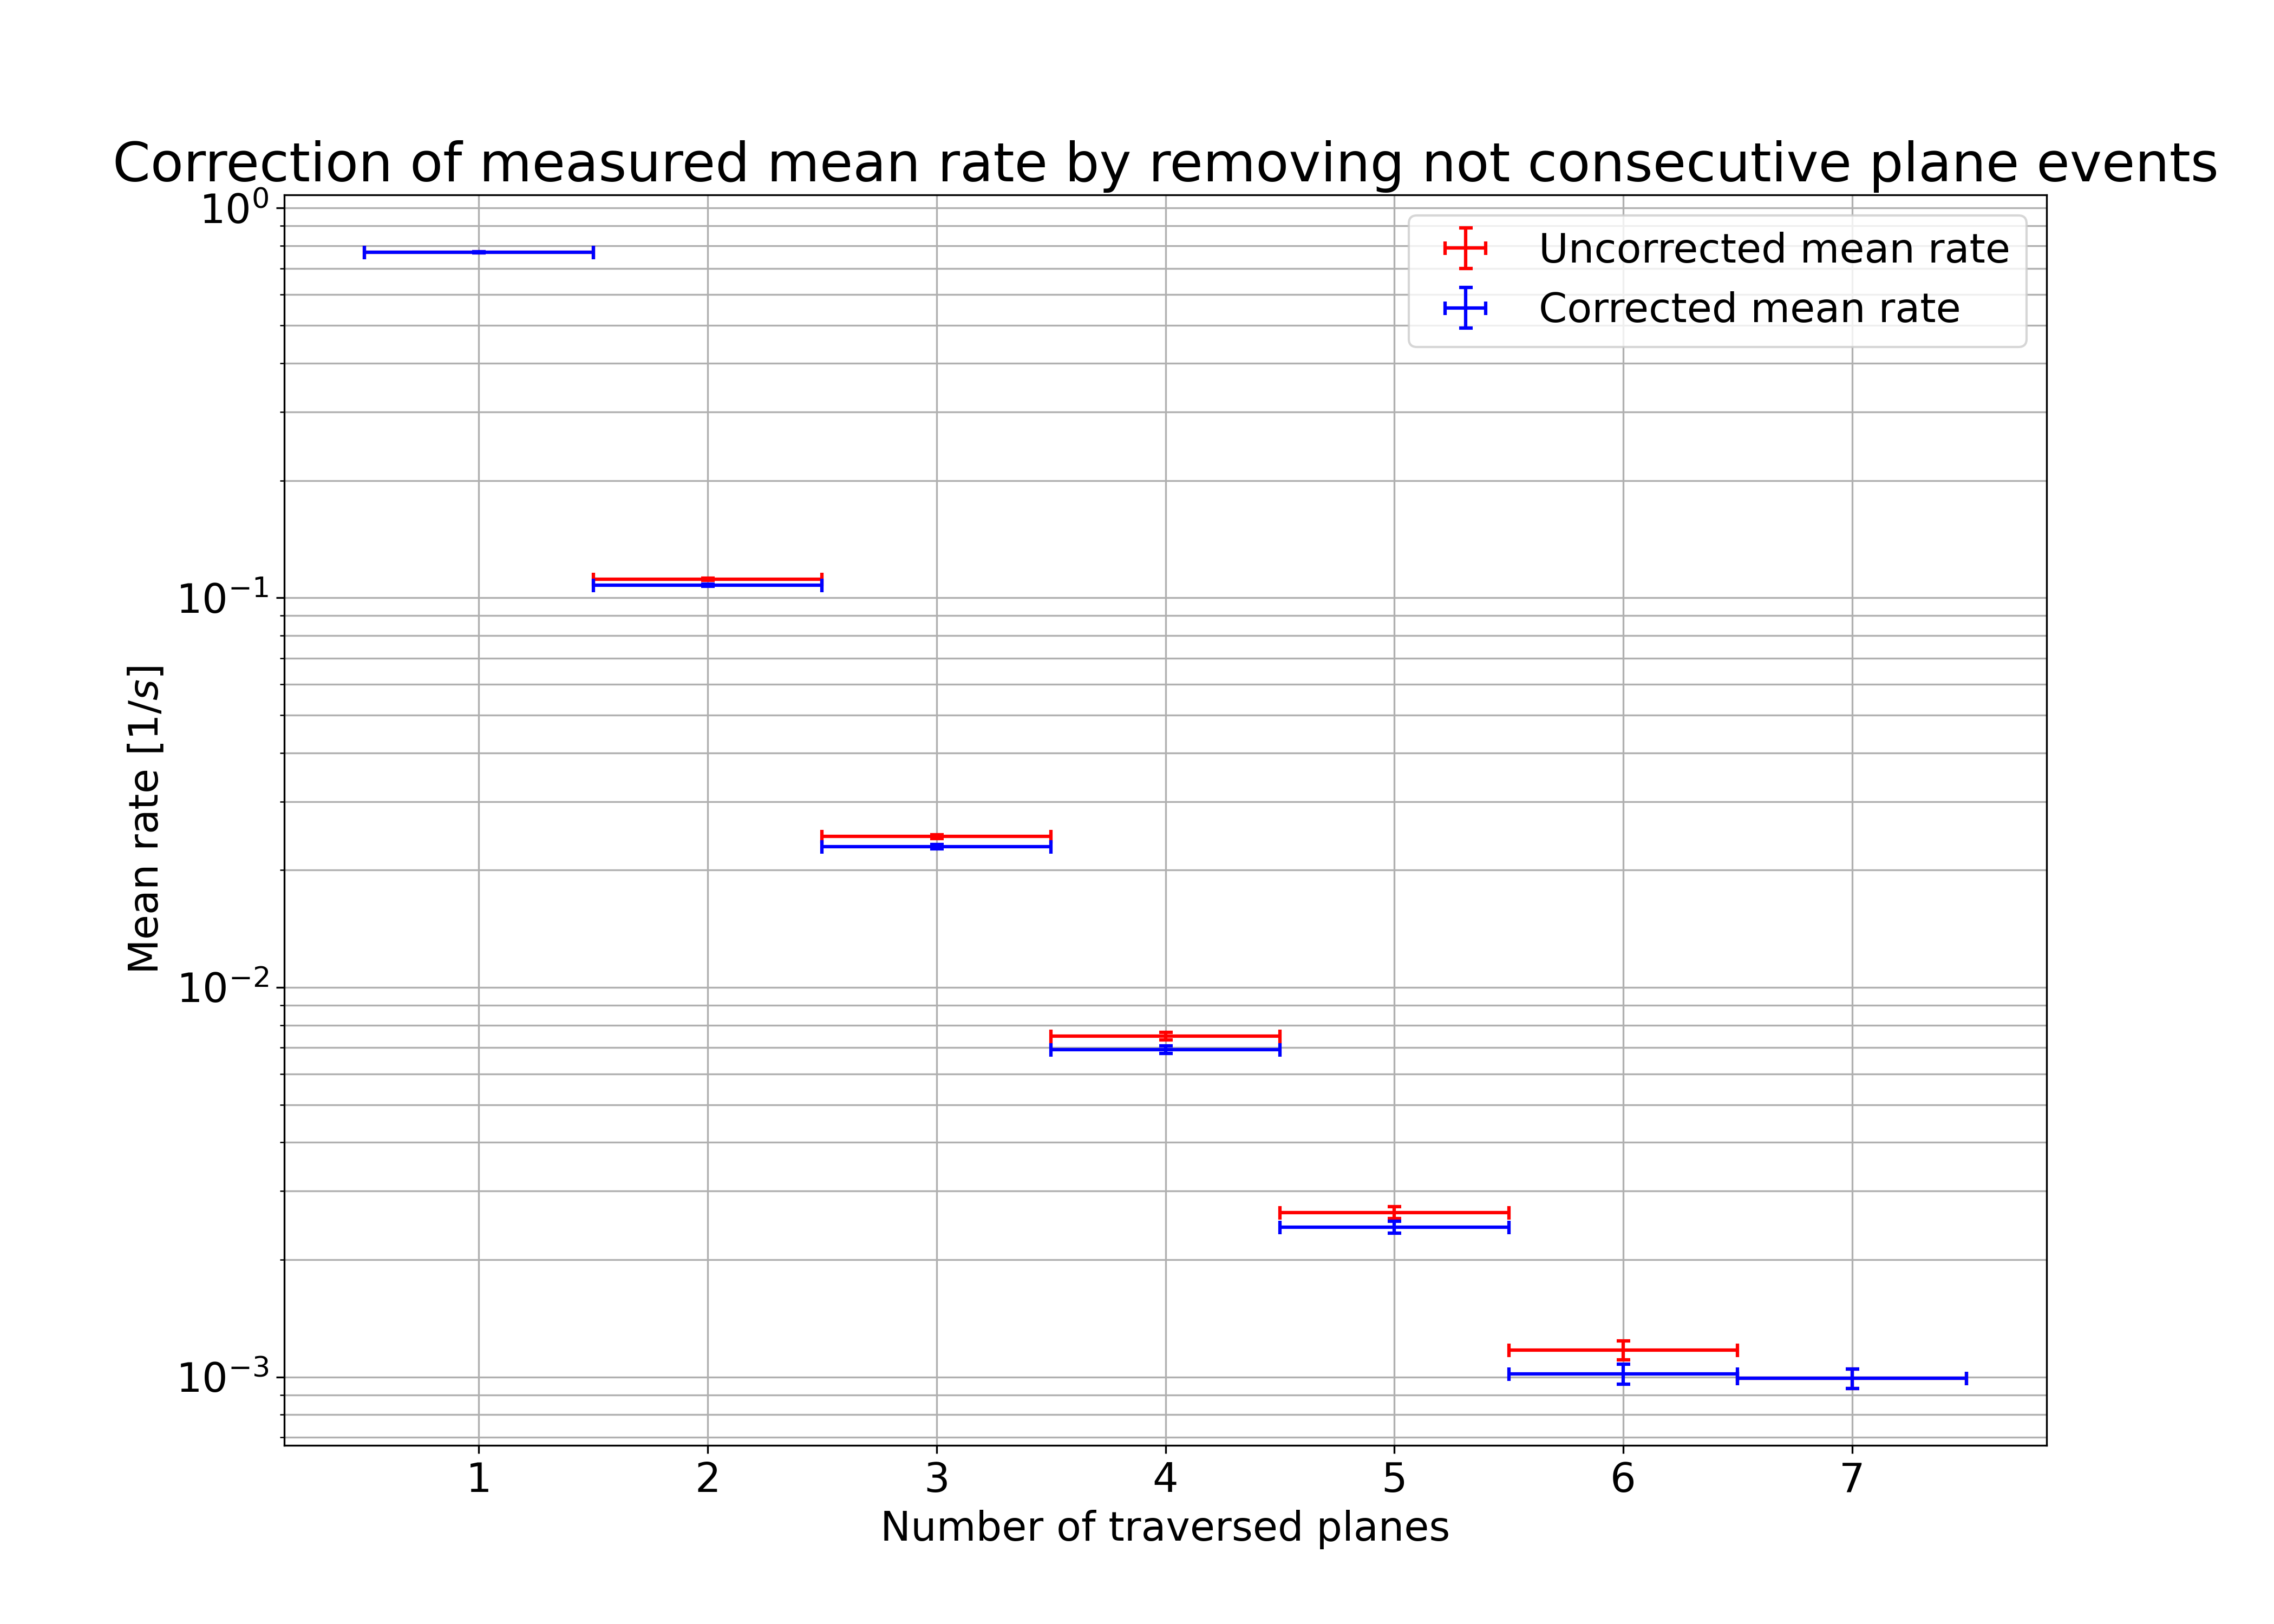
\includegraphics[width=.6\textwidth]{rate_correction}
    \caption{Mean rate correction by non-consecutive events}
  \end{figure}
\end{frame}

\begin{frame}{Cosmic Analysis}
  \LARGE track analysis \normalsize \\[.1cm]
  \begin{itemize}
    \item Alignment with data of testbeam june 2020
    \item Track visualized with 2-dimensional projection
    \item possibility to classify events as valid or fake track
  \end{itemize}
  \begin{figure}[H]
    \centering
    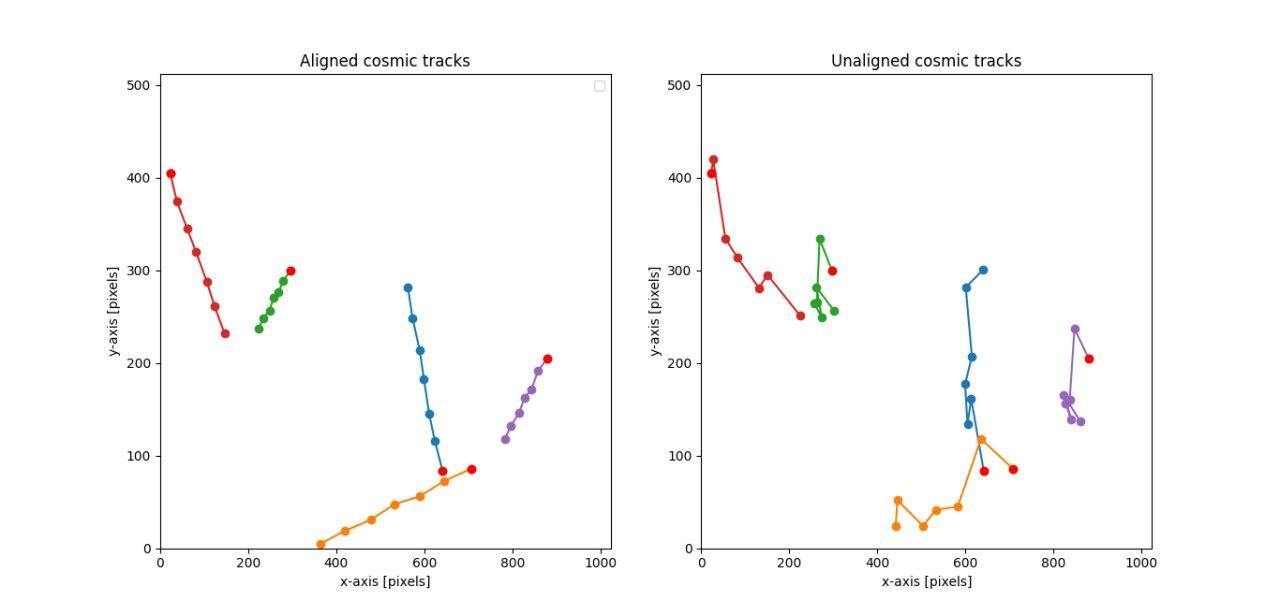
\includegraphics[width=.8\textwidth]{track_visual}
    \caption{Alignment with testbeam 2020 data}
  \end{figure}
\end{frame}

\begin{frame}{Cosmic Analysis}
  \LARGE track analysis \normalsize \\[.1cm]
  \begin{itemize}
    \item Fitting the 2D-track projections
    \item Analysis of $\chi^2_{red}$-distribution and angular distribution
    \item still open
  \end{itemize}
  \begin{figure}[H]
    \centering
    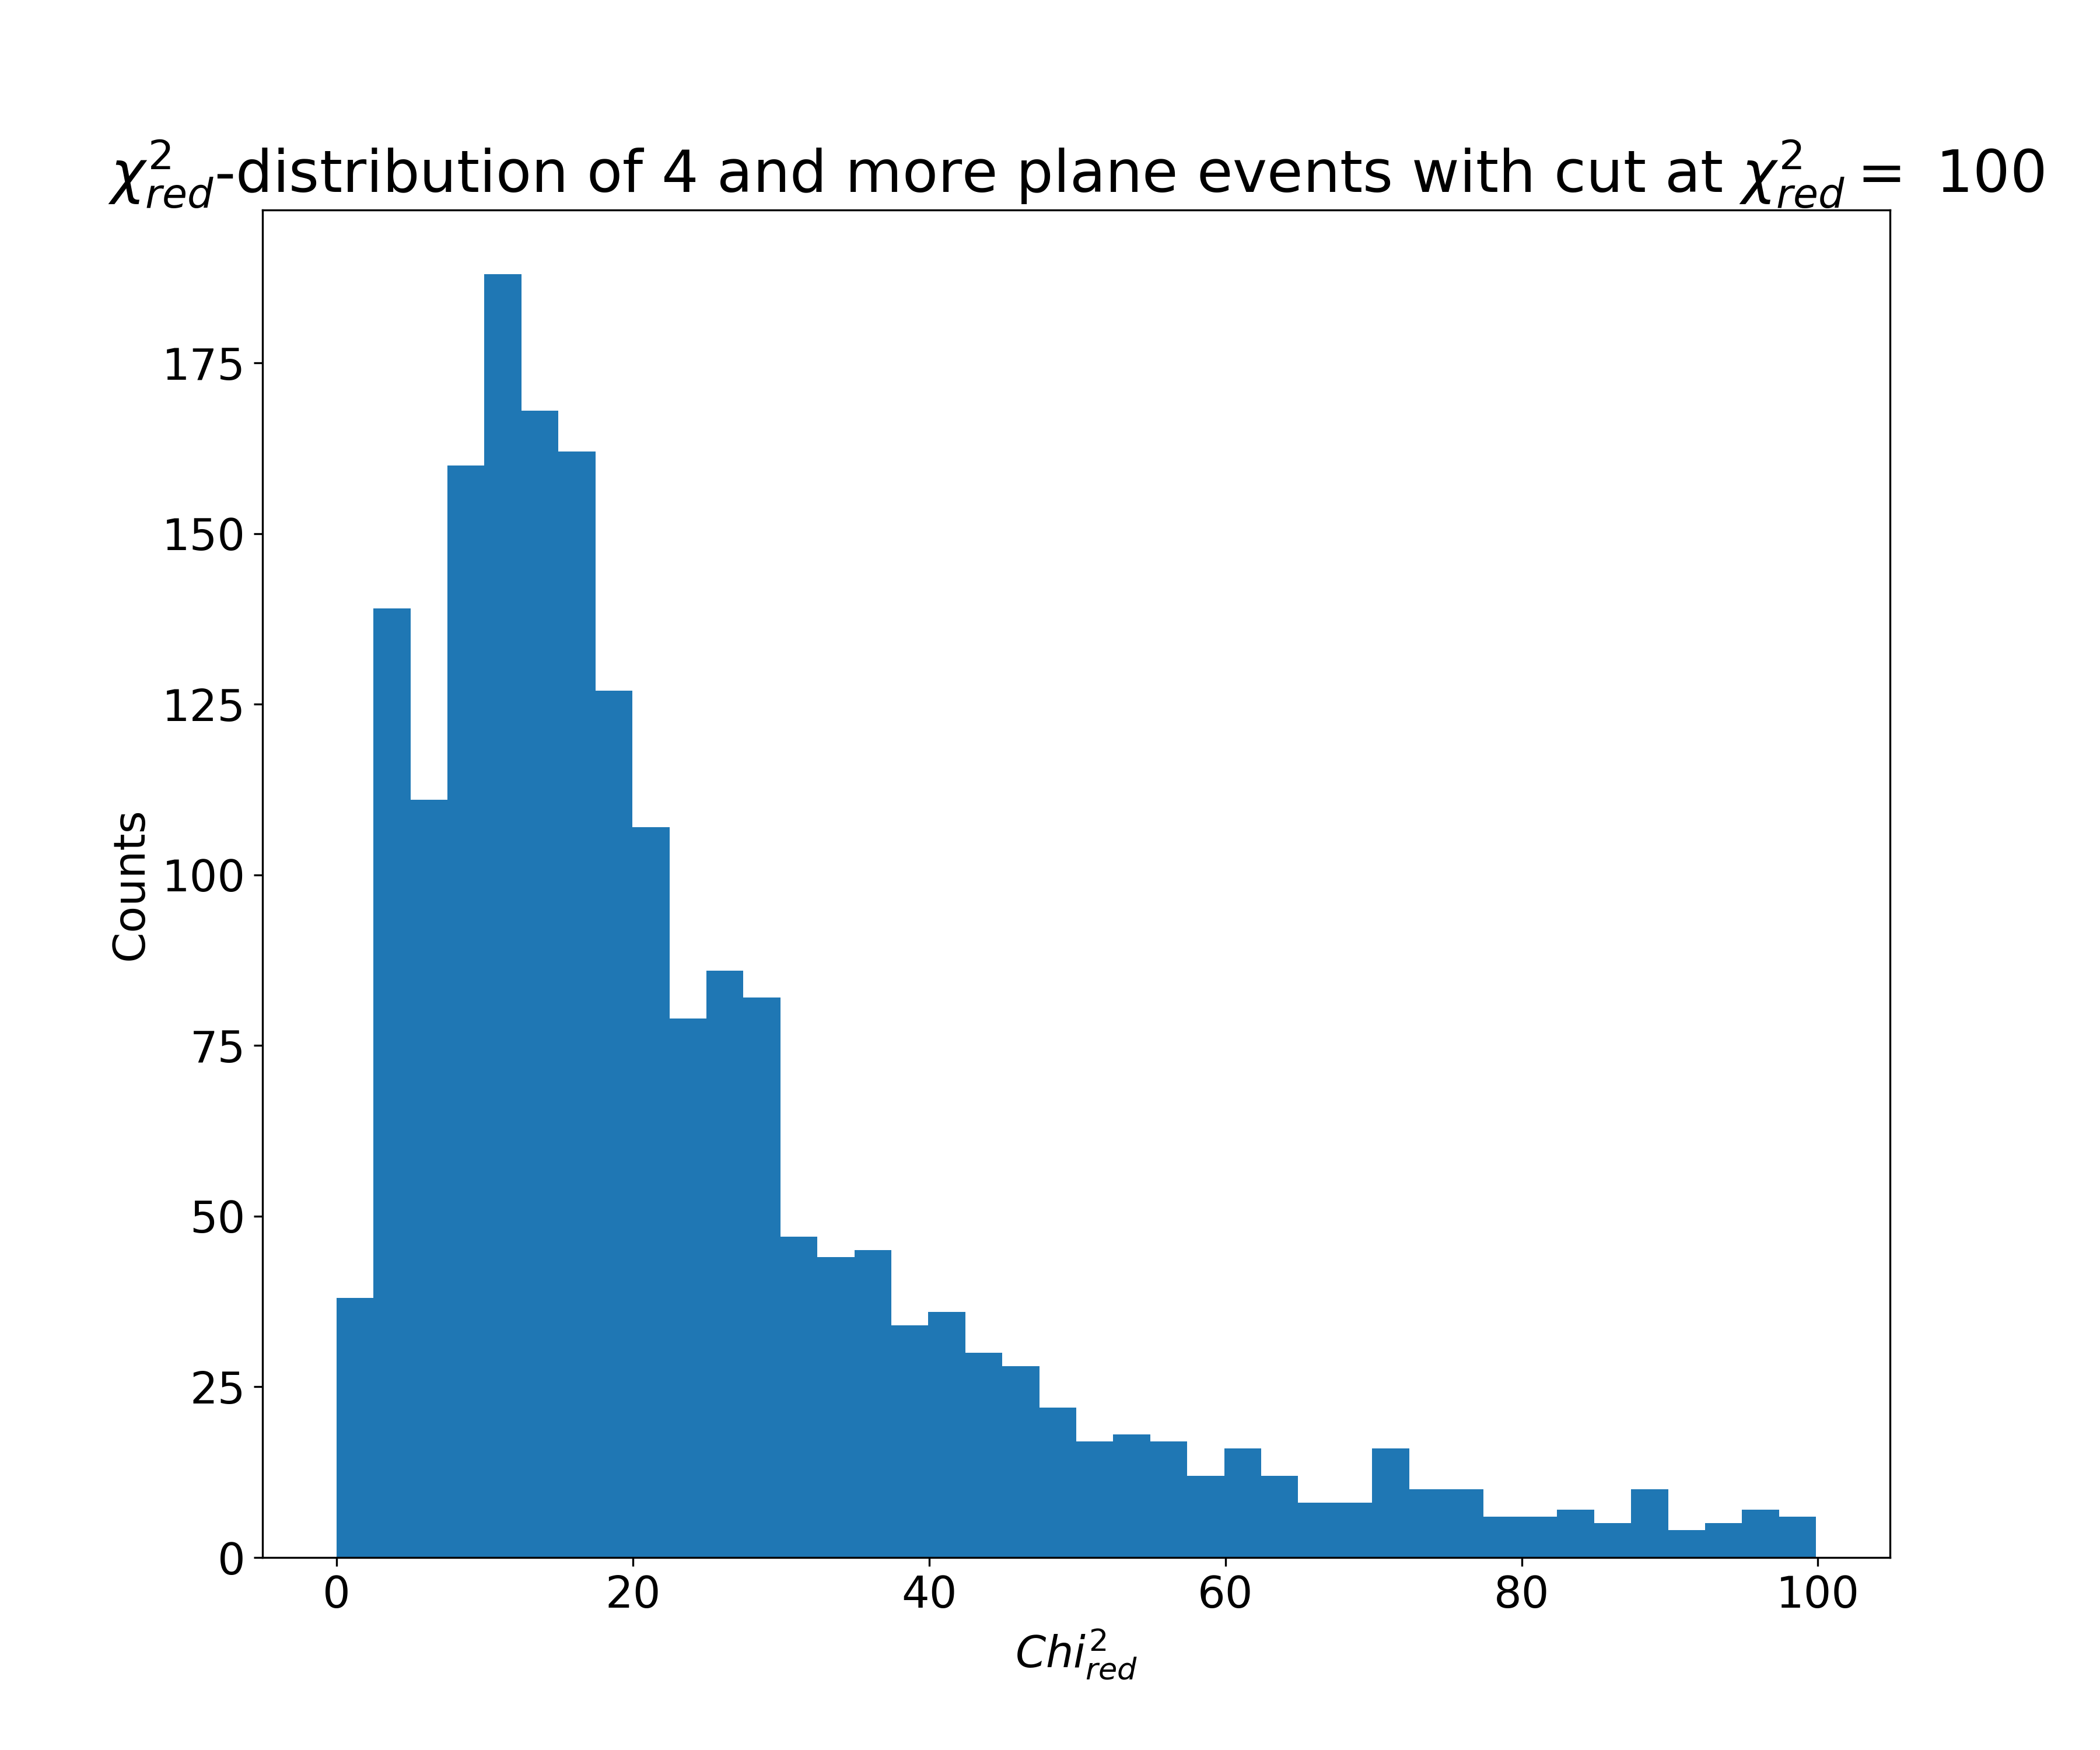
\includegraphics[width=.49\textwidth]{track_chi}
    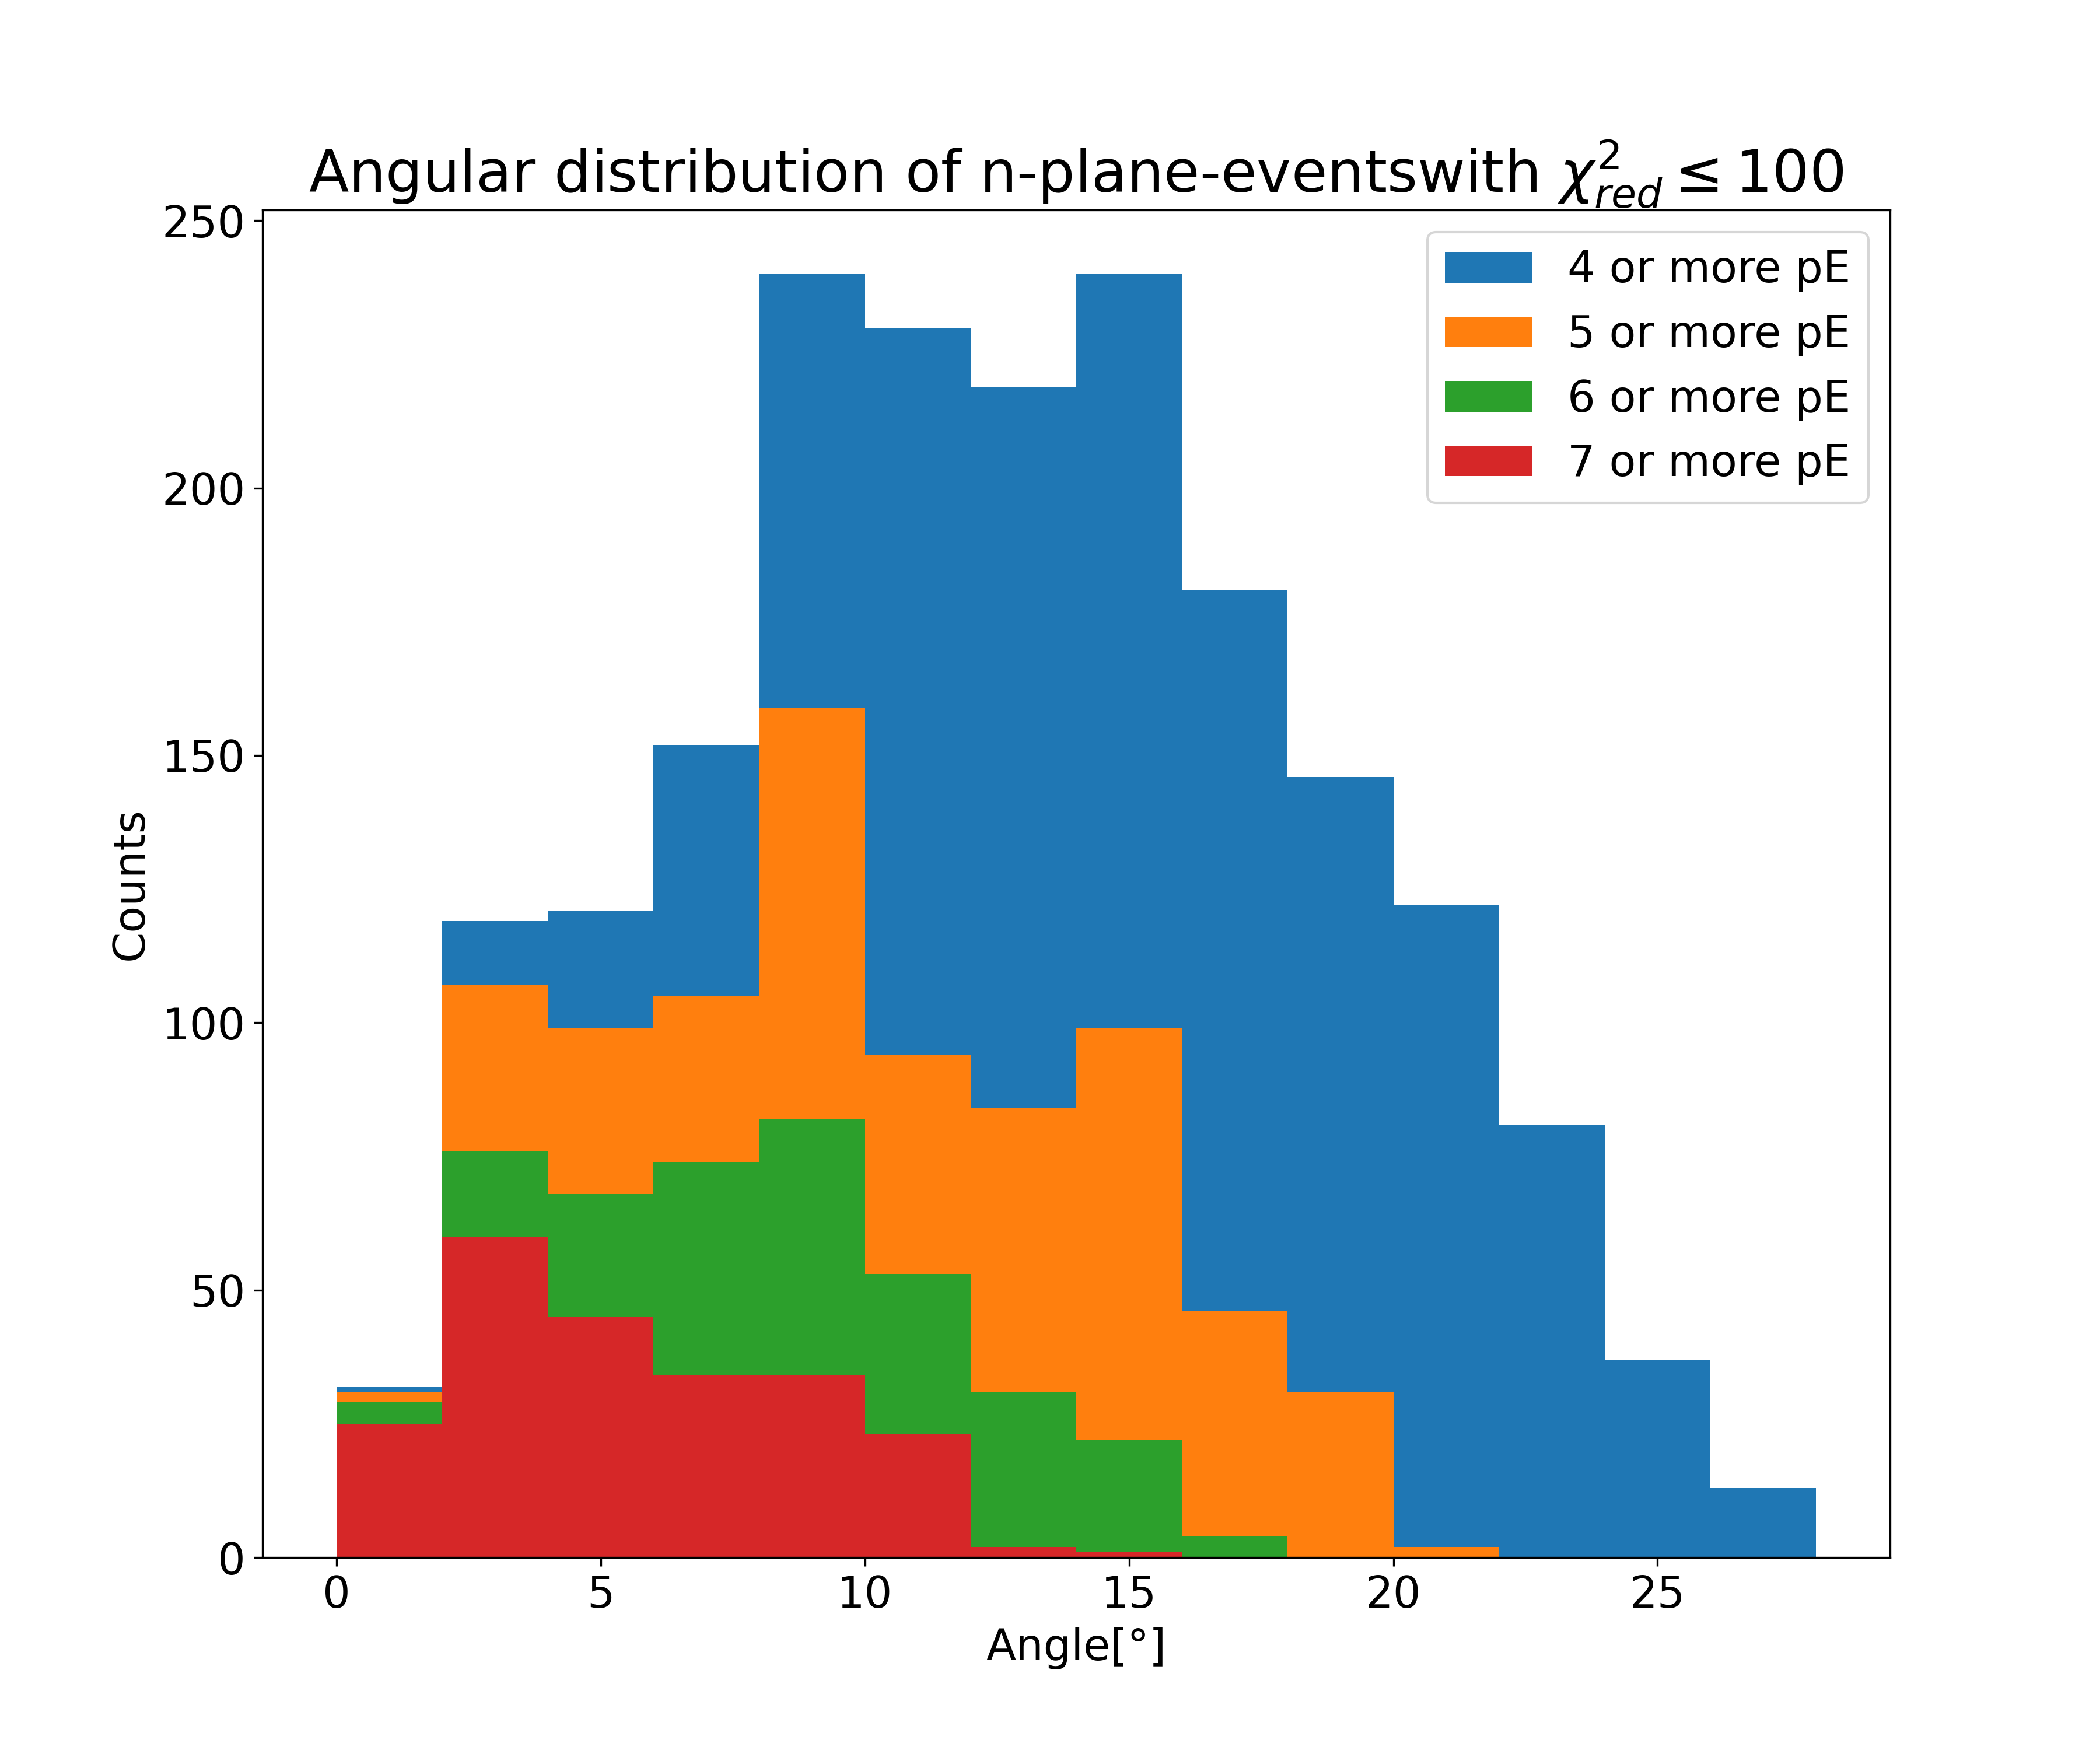
\includegraphics[width=.49\textwidth]{track_angle}
  \end{figure}
\end{frame}

\begin{frame}{Outlook}
    \begin{minipage}{.44\textwidth}
	\LARGE Projects \normalsize \\
	\begin{itemize}
	    \item Alignment \\[5pt]
		\begin{itemize} \tiny 
		    \item Trying to achieve better alignment by
			iterative track fitting (similar to corryvreckan)
		\end{itemize}
	    \item Cosmic Analysis for Thesis \\[5pt]
		\begin{itemize} \tiny 
		    \item Comparing angular distribution and rate with
			theoretical calculations
		    \item Looking at cluster sizes and charge deposit
		\end{itemize}
	    \item The ALPIDE-Telescope \\[5pt]
		\begin{itemize} \tiny 
		    \item Now have scintillators again
		    \item Trying to revive the setup in triggered mode
		       	(now together)
		    \item As of right now: Eudaq not able to work with low
			particle rate (maybe you have some input?)
		\end{itemize}
	
	\end{itemize}
    \end{minipage}
    \begin{minipage}{.55\textwidth}
	\begin{figure}[H]
	    \centering
	    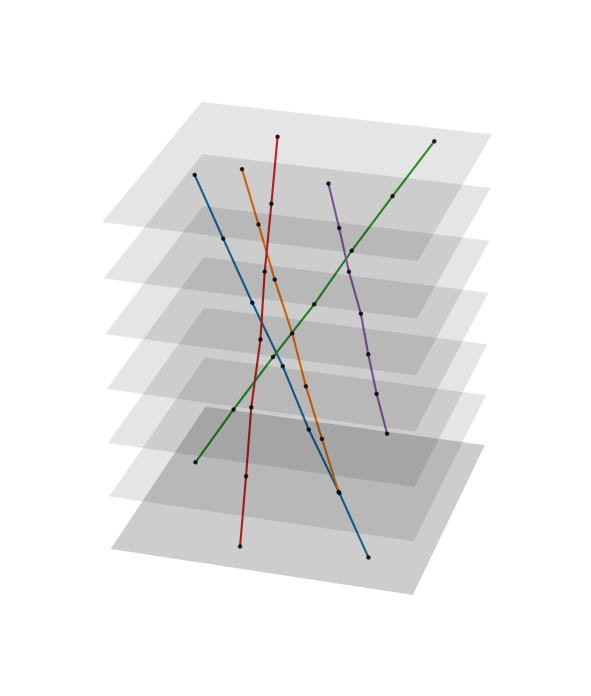
\includegraphics[width=\textwidth]{outlook.png}
	\end{figure}
    \end{minipage}
\end{frame}
\end{document}
